\section{Auswertung}
\label{sec:Auswertung}

\subsection{Bestimmung der freien Weglänge}
Zunächst werden sowohl die Sättigungsdampfdrücke $p_{\text{sätt}}$ aus \autoref{eqn:p1}, als auch die mittleren Weglängen der Elektronen $\bar{w}$ aus \autoref{eqn:w1}
für die verschiedenen Temperaturen, bei denen die Versuche durchgeführt werden, bestimmt.
Die Ergebnisse sind in \autoref{tab:f0} angegeben.



  %%%%%
  \begin{table}[H]
    \centering
    \caption{Sättigungsdampfdruck, mittlere freie Weglänge und der zusammen mit $a$ resultierende Faktor.}
    \label{tab:f0}
    \begin{tabular}{cccc}
        \toprule
        T/\si{\kelvin} & $p_{\text{sät}}$/\si{\m\bar} & $\bar{w}$/\si{\cm} & Faktor $\frac{a}{\bar{w}}$\\
        \midrule
        300 & 0,006114 & 0,4743212 & 2,1083\\ % $1,79~~~$
        420 & 4,2692 & 0,0006793 & 1472,10\\
        440 & 8,9851 & 0,0003227 & 3098,85\\
        460 & 17,7257 & 0,0001636 & 6112,47\\
        \bottomrule
    \end{tabular}
\end{table}
%%%%%

\noindent
Der Abstand zwischen Kathode und Beschleunigungselektrode beträgt bei der verwendeten Apparatur etwa $\SI{1}{\centi\metre}$.
Daraus folgt, dass die mittlere Weglänge im Mikrometerbereich liegen sollte.
Es können demnach gute Franck-Hertz-Kurven bei Temperaturen von $\SI{400}{\kelvin}$ bis $\SI{450}{\kelvin}$ aufgezeichnet werden.

%%%%%

\subsection{Integrale Energieverteilung}
\label{sec:ie}
Wie bereits in der Durchführung erläutert wird eine feste Beschleunigungsspannung von $U_b = \SI{11}{\volt}$ eingestellt und der Auffängerstrom gemessen.
Um nun die integrale Energieverteilung bestimmen zu können, müssen mehrere Spannungswerte $U_a$ gegen den dazugehörigen Wert
\begin{equation}
  \increment I_a \coloneq I_a(U_a) - I_a(U_a + \increment U_a)
\end{equation}
aufgetragen werden.
Dieser Zusammenhang beschriebt nach \autoref{eqn:beschlGl} die Energieverteilung. Eine hohe Änderung von $I_a$ entspricht einer hohen Anzahl von Elektronen,
die eben diese kinetische Energie besitzen und nun durch die Bremsspannung aufgehalten werden.
\newline
Die Messungen wurden einmal bei Raumtemperatur und einmal bei $T = \SI{423,16}{\kelvin}$ durchgeführt. Die Ergebnisse sind für Raumtemperatur in \autoref{fig:ev1} und für
$T = \SI{423,16}{\kelvin}$ in \autoref{fig:ev2} dargestellt.

\begin{figure}[H]
	\centering
	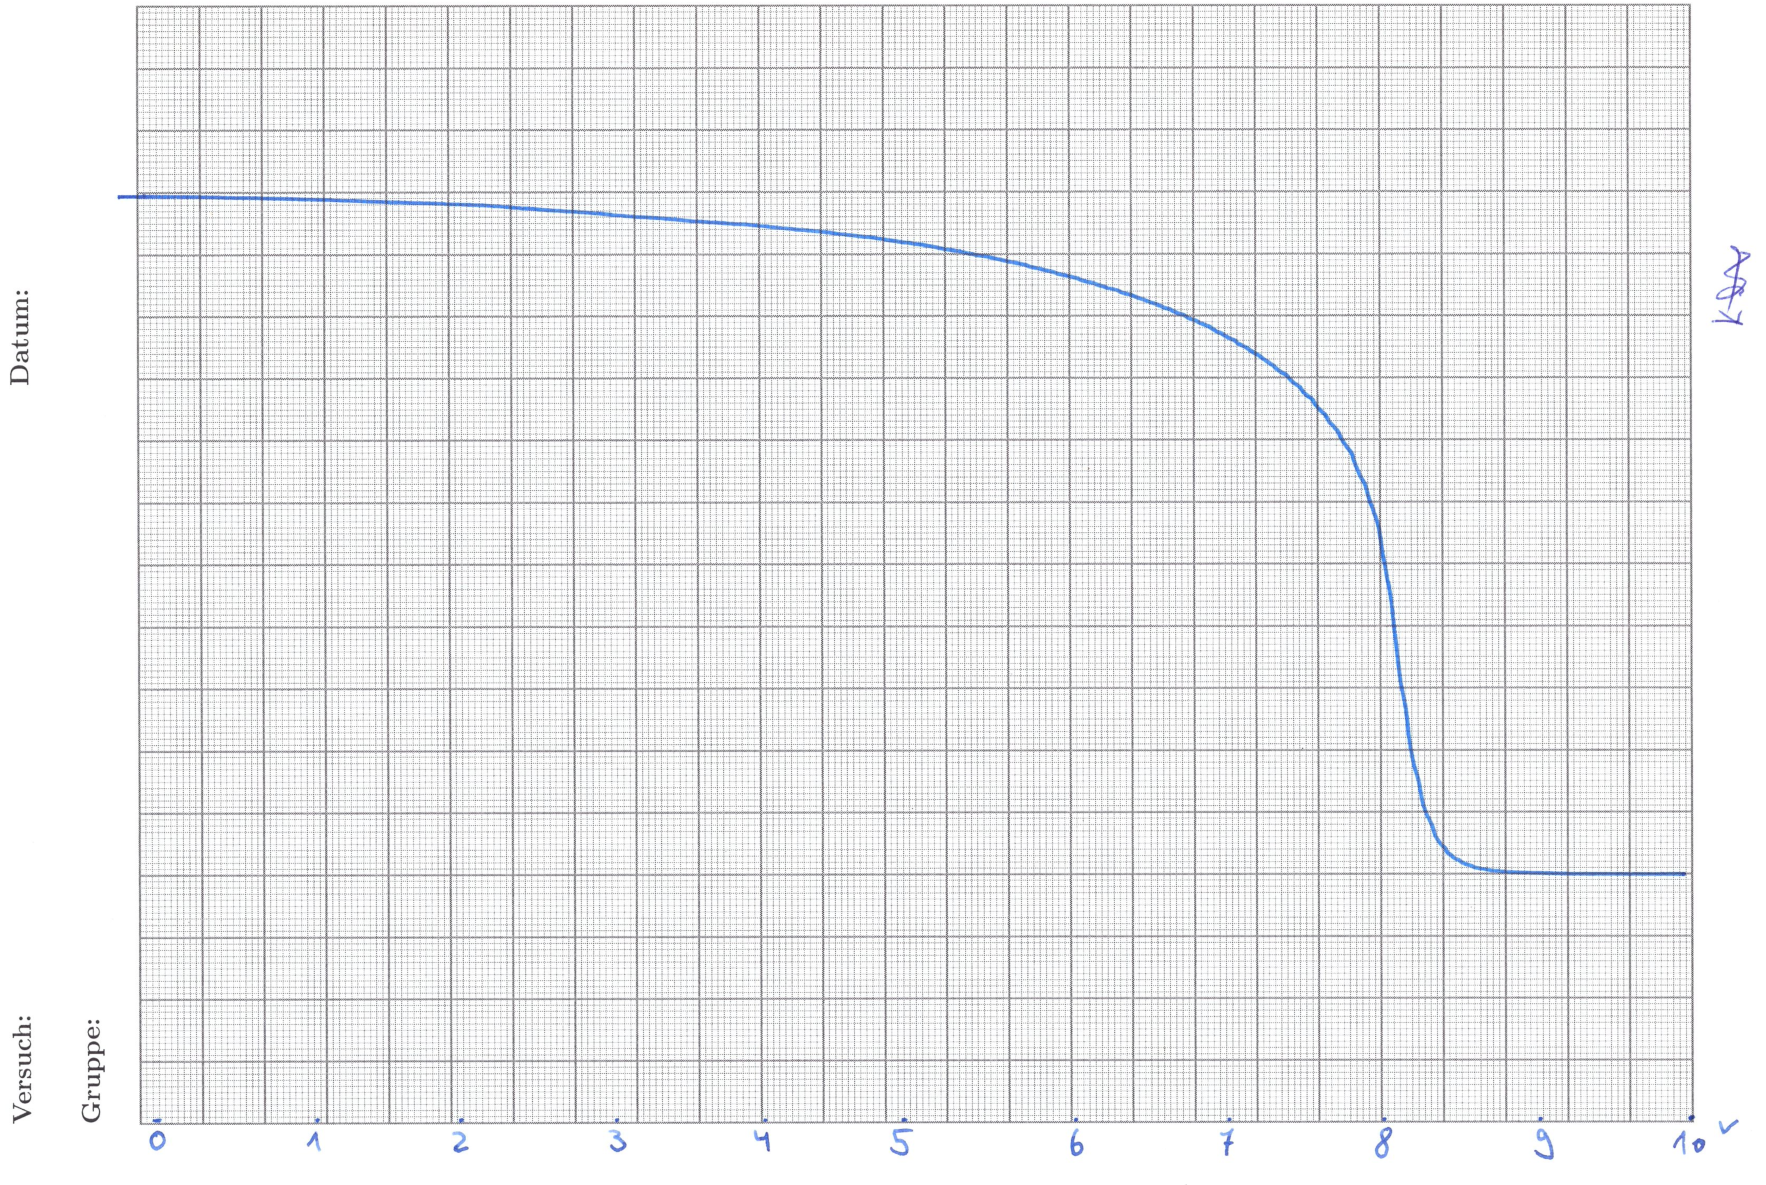
\includegraphics[width=0.7\linewidth]{data/EnergieverteilungRT.png}
	\caption{Energieverteilungsmessung bei Raumtemperatur.}
	\label{fig:ev1}
\end{figure}

\begin{figure}[H]
	\centering
	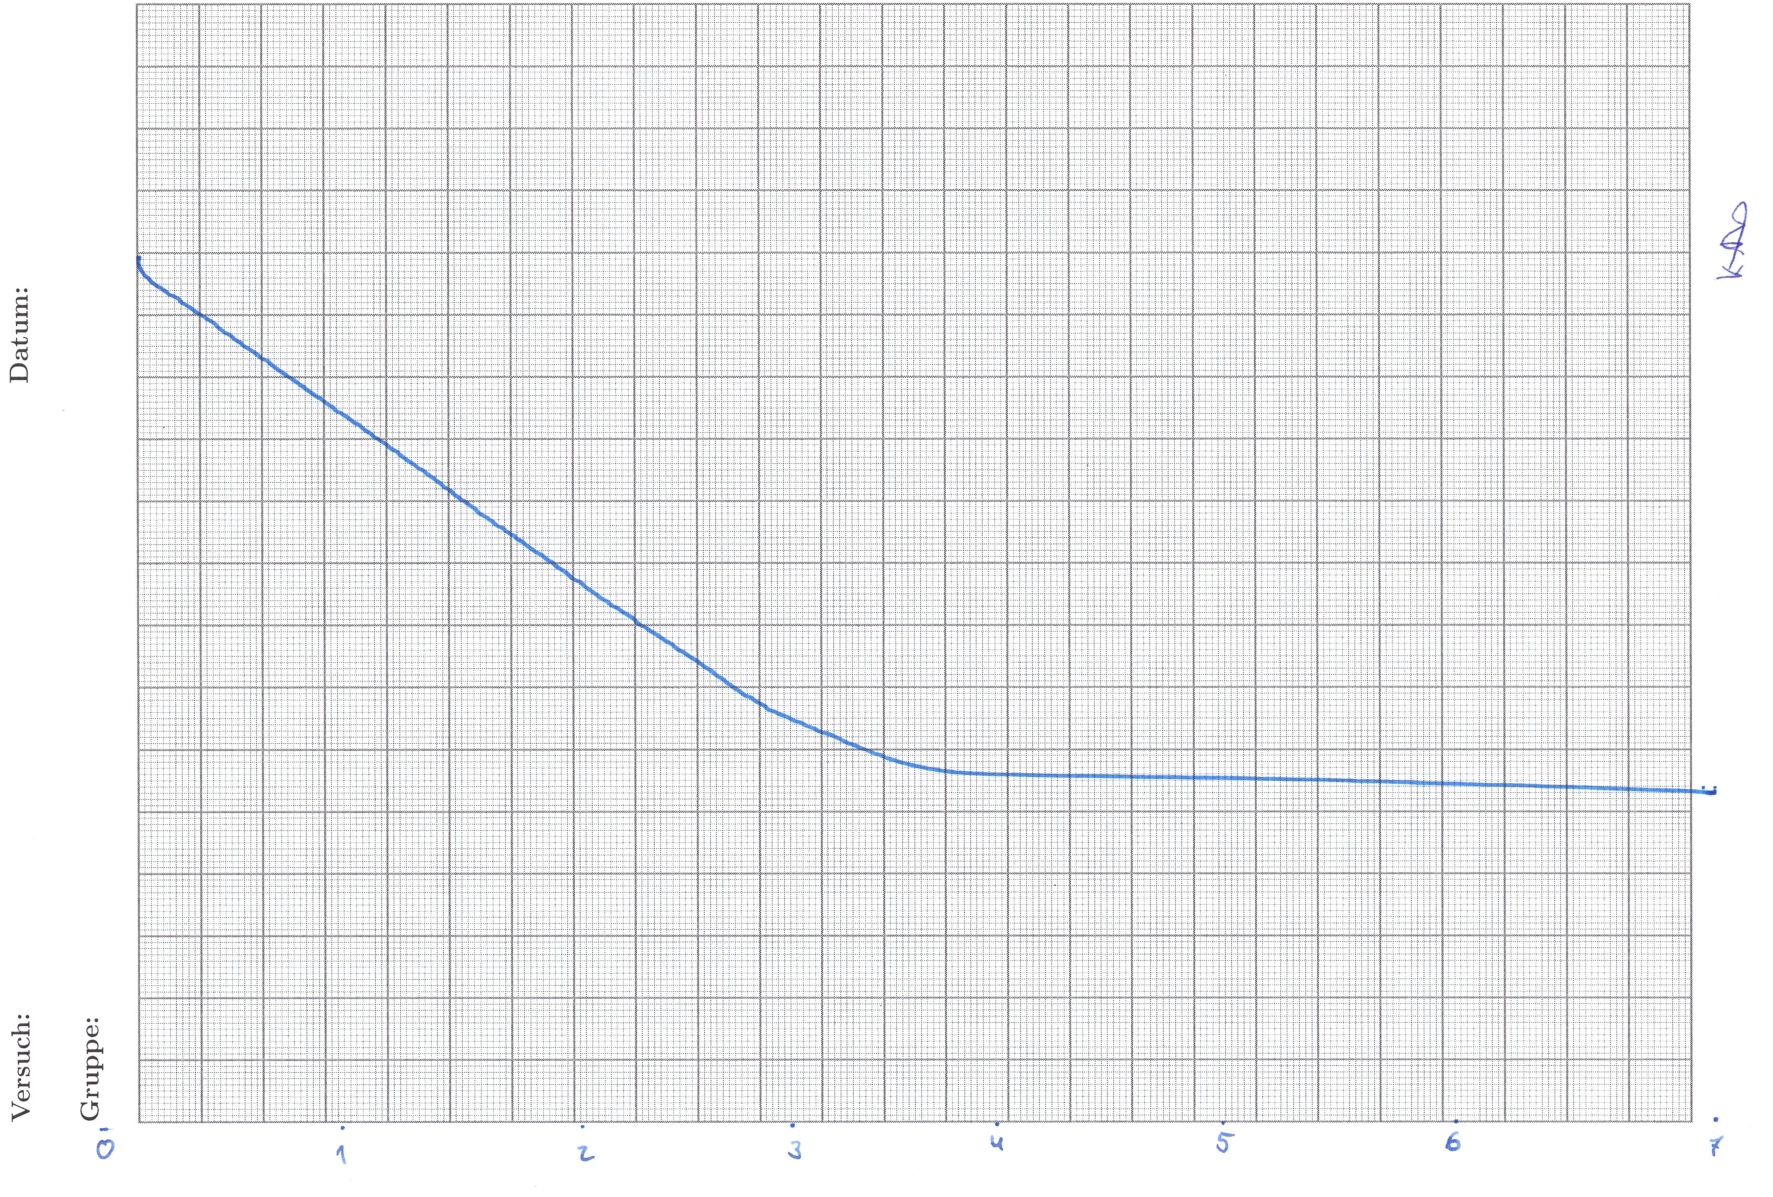
\includegraphics[width=0.7\linewidth]{data/Energieverteilung150C.png}
	\caption{Energieverteilungsmessung bei $T = \SI{423,16}{\kelvin}$.}
	\label{fig:ev2}
\end{figure}

\newpage
Der Graph der Differenz $I_A(U_A+\upDelta U_A)-I_A(U_A)$ ist in \autoref{fig:diff} zu sehen.
\begin{figure}[H]
    \centering
    \includegraphics{build/Differenz.pdf}
    \caption{Differenz $I_A(U_A+\upDelta U_A)-I_A(U_A)$ gegen die Spannung $U_A$.}
    \label{fig:diff}
\end{figure}

\noindent
An den Differenzen bei Raumtemperatur kann nun das Minimum abgelesen werden. Es liegt bei $8\si{\V}$ und ist bereits rot makiert.
Mit Hilfe dieses Minimums, dass $U_{\text{B,eff}}$ aus \autoref{eqn:potentialGef} entspricht, kann jetzt zusammen mit der eingestellten Beschleunigungsspannung
$U_B=11\si{\V}$ und \autoref{eqn:kont} das Kontaktpotential berechnet werden. Es hat den Wert
\begin{equation*}
    K=3\si{\V}.
\end{equation*}


\subsection{Interpretation der Franck-Hertz Kurven}
Die Franck-Hertz-Kurve bei $T = \SI{443,16}{\kelvin}$ ist in \autoref{fig:fh170} und die bei $T = \SI{463,16}{\kelvin}$ in \autoref{fig:fh190} aufgezeichnet.
\begin{figure}[H]
	\centering
	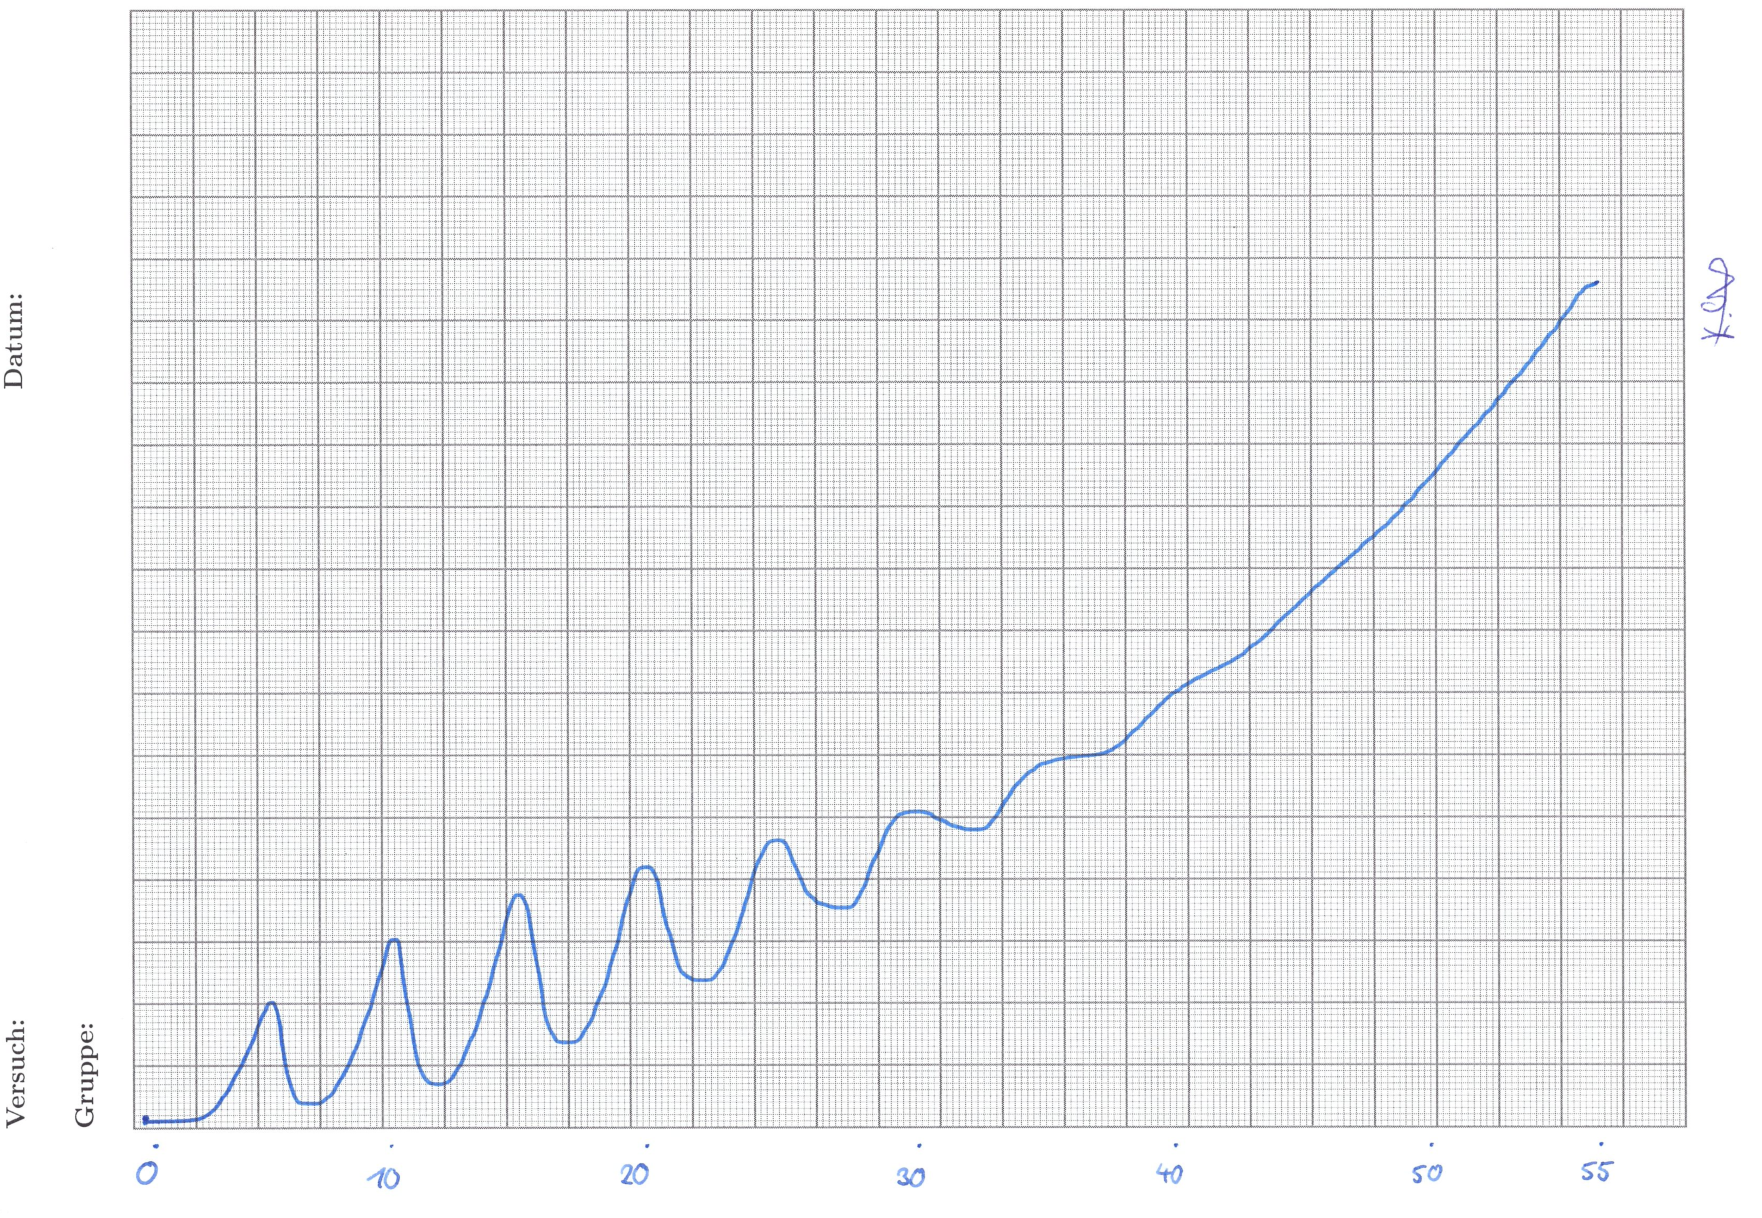
\includegraphics[width=0.7\linewidth]{data/Franck-Hertz170C.png}
	\caption{Franck-Hertz-Kurve bei $\SI{443,16}{\kelvin}$.}
	\label{fig:fh170}
\end{figure}

\noindent
Die ablesbaren Maxima der Franck-Hertz-Kurve bei $T = \SI{443,16}{\kelvin}$ befinden sich bei
\begin{align*}
  U_1 &= \SI{4,25}{\volt}, \\
  U_2 &= \SI{8,97}{\volt}, \\
  U_3 &= \SI{13,69}{\volt},\\
  U_4 &= \SI{18,64}{\volt},\\
  U_5 &= \SI{23,61}{\volt}.
\end{align*}
\noindent
Daraus folgt als gemittelter Abstand der Maxima
\begin{align*}
  \upDelta U &= \SI{4,84 \pm 0,12}{\volt}.
\end{align*}

\begin{figure}[H]
	\centering
	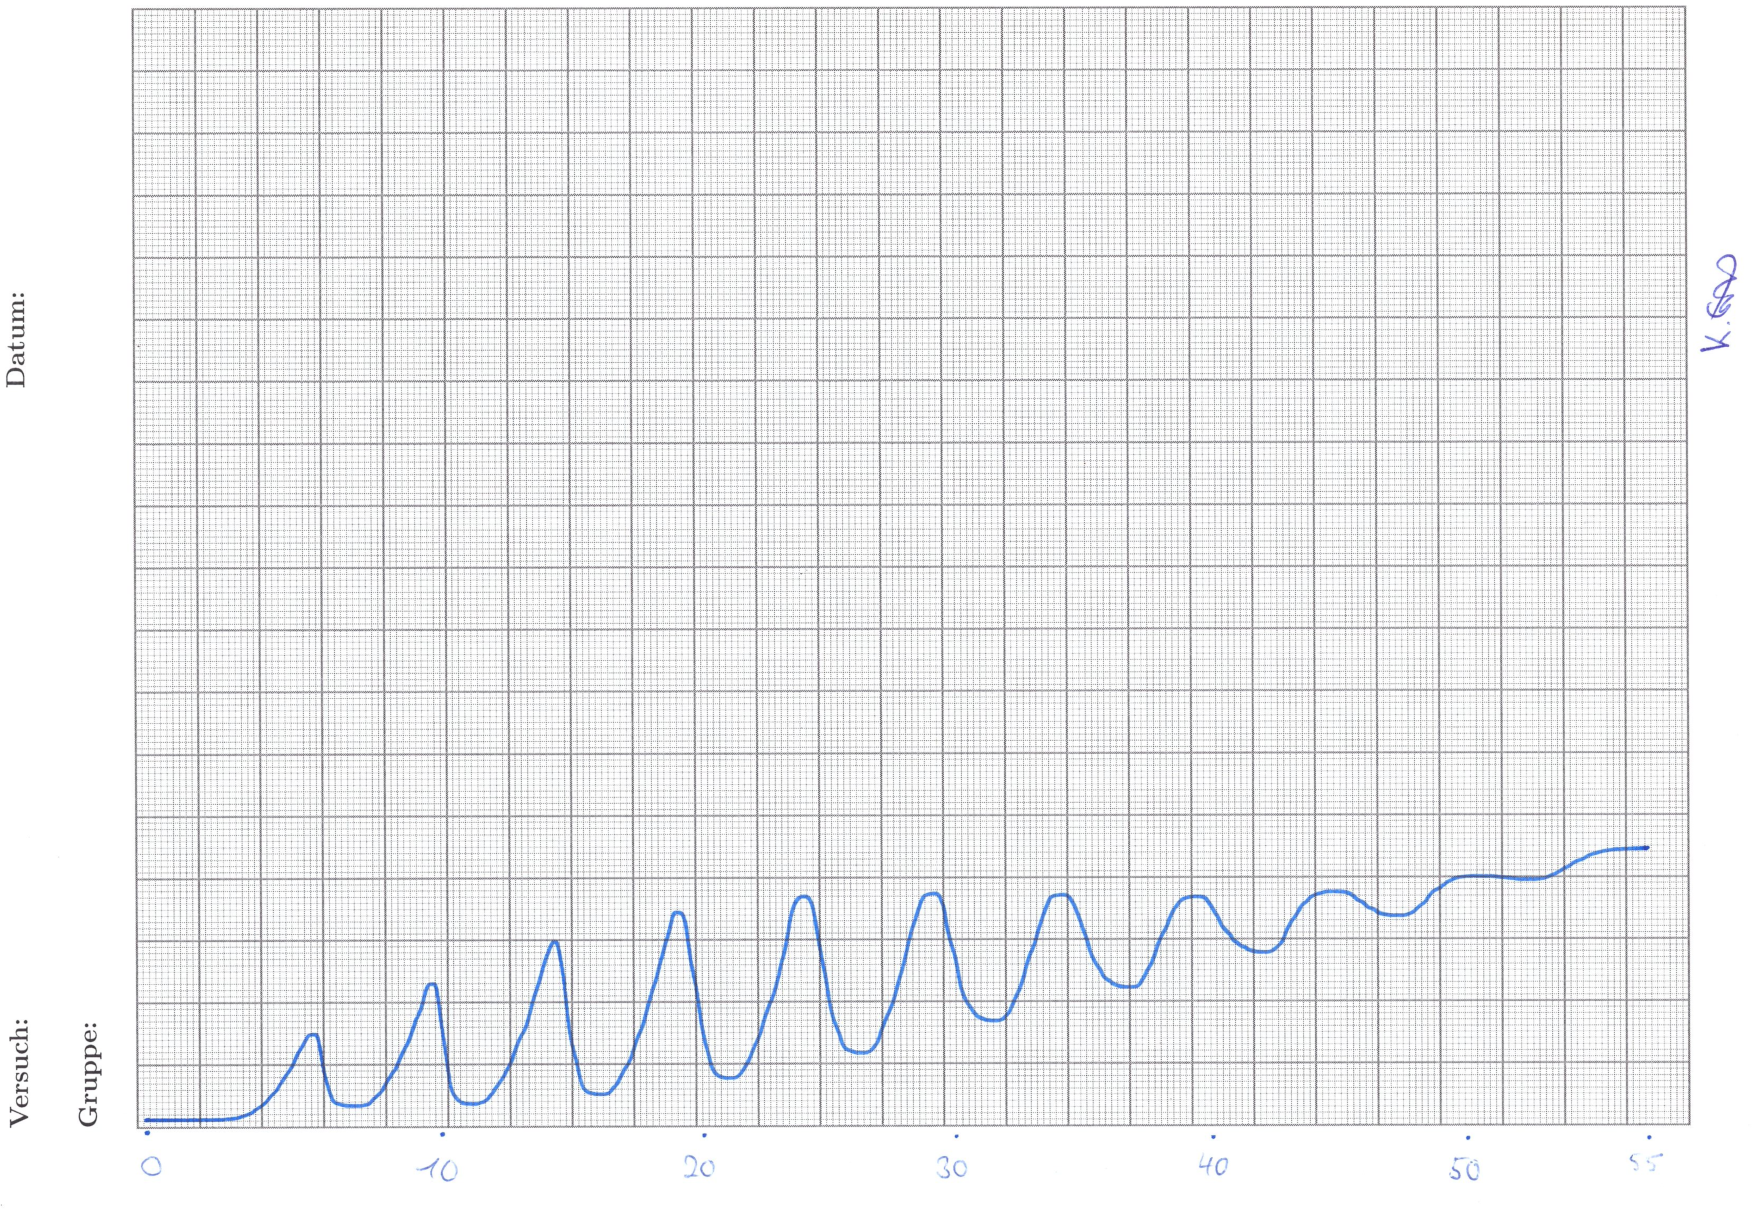
\includegraphics[width=0.7\linewidth]{data/Franck-Hertz190C.png}
	\caption{Franck-Hertz-Kurve bei $\SI{463,16}{\kelvin}$.}
	\label{fig:fh190}
\end{figure}
\noindent
Die ablesbaren Maxima der Franck-Hertz-Kurve bei $T = \SI{463,16}{\kelvin}$ befinden sich bei
\begin{align*}
  U_1 &= \SI{6,34}{\volt}, \\
  U_2 &= \SI{10,98}{\volt}, \\
  U_3 &= \SI{15,85}{\volt},\\
  U_4 &= \SI{20,73}{\volt},\\
  U_5 &= \SI{25,61}{\volt},\\
  U_6 &= \SI{30,73}{\volt}.
\end{align*}
\noindent
Daraus folgt als gemittelte Abstand der Maxima
\begin{align*}
  \upDelta U &= \SI{4,88 \pm 0,15}{\volt}.
\end{align*}

\noindent
Es ergibt sich als aus beiden Messungen gemittelter Wert
\begin{align*}
  \upDelta U &= \SI{4,86 \pm 0,14}{\volt}.
\end{align*}

\noindent
Nach \autoref{eqn:hfu} beträgt die Wellenlänge $\lambda$ der emittierten Strahlung somit
\begin{align*}
  \lambda &= \SI{255+-4}{\nano\metre}.
\end{align*}